\section{Datasets}\label{section:datasets}

For verifying our initial proposals, we envisioned a set of experiments on real world datasets. We decided to use at least two data sources with significant previous usage in the literature, so we could easily compare our results to previous experiments. 

In addition, we wanted to see our proposed methods fares in tag prediction tasks in datasets with different characteristics. We took into account dataset metrics such as the average number of tags assigned to each resource, total number of resource, total number of unique tags, and so on.

\subsection{Dataset 1: Delicious t-140}\label{subsec:dataset_1}

This dataset has been created during June 2008 for \cite{zubiaga_etal_2009}, for the task of Content-based Clustering.

\subsubsection{Construction}

This dataset was constructed using by subscribing to the 140 most popular tags on the Delicious.com website\footnote{Delicious was a popular online bookmarking website now inactive.} between April 07, 2008 and April 12, 2008.  Every time a URL was tagged using one of these 140 tags, the corresponding HTML document would be stored in the database (along with all tags assigned to it, even if they weren't in the top 140 set).

Once this dataset was collected, all tags having occurred in less than two documents were removed (so as to abide by the website's "common tag" definition and to remove overly noisy tags). Also, webpages written in languages other than English were also removed from the dataset.

After these initial steps, the dataset totalled 144,574 unique documents and 67,104 unique tags.

\subsubsection{Preprocessing}

Following literature conventions, we added a few pruning and preprocessing steps to this dataset, so as to make it more amenable to training models on.

We removed documents that had only been tagged with a single unique tag. We also removed from the dataset all documents which has been tagged by only a single user.

More importantly, we removed from the dataset all tags which had been used in less than 10 separate documents.\footnote{Such \textit{tag-pruning} reflects standard practice in many works dealing with tag prediction, especially as related to broad folksonomies.}

These pruning steps brought the total number of documents down to 143,716 and the number of distinct tags to 9,184.

As for text preprocessing, we normalized all tags by applying lowercasing and removing special characters.

The textual contents consisted of HTML pages. Once more following literature convention, we removed HTML tags to arrive at a \textit{clean} version of the dataset.

\renewcommand{\arraystretch}{1.5}

\begin{table}[!h]
\centering
\caption{Dataset Statistics: Delicious t-140 (after pruning and preprocessing)}
\begin{tabular}{|c|c|}
\hline
\specialcell{Total number of Resources} & \,\,\, 147,716 \\
\hline
\specialcell{Total number of unique tags} & \,\,\, 9,184 \\
\hline
\specialcell{Average number of tags per resource} & \,\,\, 13.12 \\
\hline
\specialcell{Minimum number of tags per resource} & \,\,\, 1 \\
\hline
\specialcell{Maximum number of tags per resource} & \,\,\, 25 \\
\hline
\specialcell{Average number of resources per tag} & \,\,\, 205.24 \\
\hline
\specialcell{Minimum number of resources per tag} & \,\,\, 10 \\
\hline
\specialcell{Maximum number of resources per tag} & \,\,\, 26,603 \\
\hline
\end{tabular}
\label{tab:dataset_statistics_delicious}
\end{table}

\begin{figure}[!h]
    \centering
    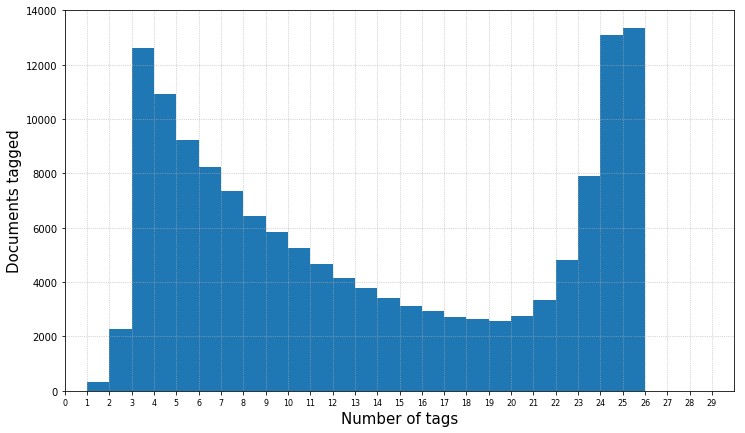
\includegraphics[width=\textwidth]{chapters/05_experiments/images/delicious_tag_per_resource.png}
    \caption{Distribution of the number of unique tags assigned to each document in the Delicious t-140 dataset (after pruning and preprocessing).}
    \label{fig:delicious_tag_doc_distr}
\end{figure}

\begin{figure}[H]
    \centering
    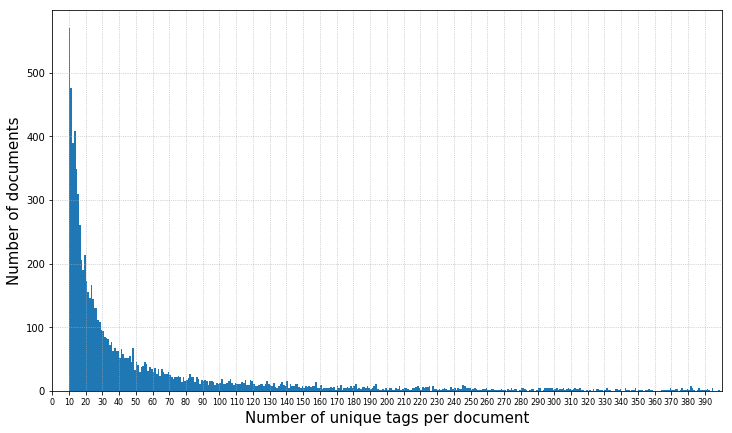
\includegraphics[width=\textwidth]{chapters/05_experiments/images/delicious_resource_per_tag.png}
    \caption{Distribution of the number of documents each tag was assigned to in the Delicious t-140 dataset (after pruning and preprocessing, not counting multiple assignments).}
    \label{fig:delicious_tag_doc_distr}
\end{figure}

\subsection{Dataset 2: Movielens 20M + IMDB Synopses}\label{subsec:dataset_2}

For our second dataset we chose one which, as previously explained, had different characteristics compared to the first dataset. We did this to verify whether (and to what extent) our methods and other methods perform in datasets which differ with respect to metrics such as average number of tags per document, total number of tags, etc.

Once again, we wanted to choose data from sources which have been often used in the literature. With that in mind, we chose to work with a MovieLens dataset and with movie synopsis data from the International Movie Database.

While it is true that combining both datasets yields another dataset which different from the first two, there are examples in the literature \citep{peralta_2007,kataria_2016} where these two datasets were combined.

\renewcommand{\arraystretch}{1.5}


\begin{table}[H]
\centering
\caption{Dataset Statistics: MovieLens 20M + IMDB Synopses (after pruning and preprocessing)}
\begin{tabular}{|c|c|}
\hline
\specialcell{Total number of Resources} & \,\,\, 6,710 \\
\hline
\specialcell{Total number of unique tags} & \,\,\, 2,138 \\
\hline
\specialcell{Average number of tags per resource} & \,\,\, 12.21 \\
\hline
\specialcell{Minimum number of tags per resource} & \,\,\, 1 \\
\hline
\specialcell{Maximum number of tags per resource} & \,\,\, 189 \\
\hline
\specialcell{Average number of resources per tag} & \,\,\, 38.33 \\
\hline
\specialcell{Minimum number of resources per tag} & \,\,\, 10 \\
\hline
\specialcell{Maximum number of resources per tag} & \,\,\, 854\\
\hline
\end{tabular}
\label{tab:dataset_statistics_movielens}
\end{table}

\begin{figure}[H]
    \centering
    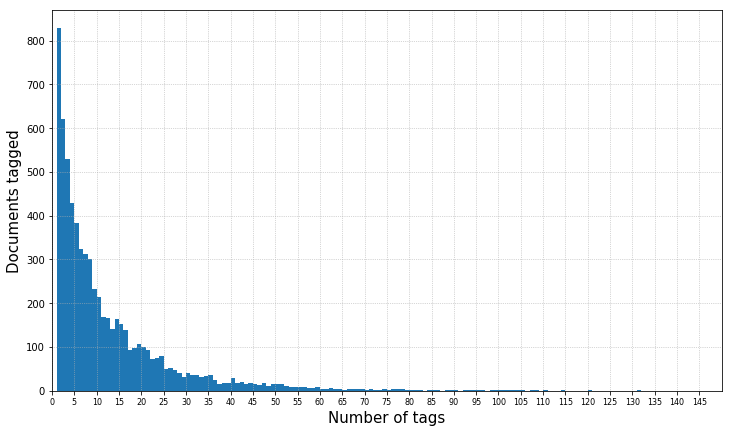
\includegraphics[width=\textwidth]{chapters/05_experiments/images/movielens_tags_per_resource.png}
    \caption{Distribution of the number of unique tags assigned to each document in the Movielens 20M + IMDB Synopses dataset (after pruning and preprocessing).}
    \label{fig:delicious_tag_doc_distr}
\end{figure}

\begin{figure}[H]
    \centering
    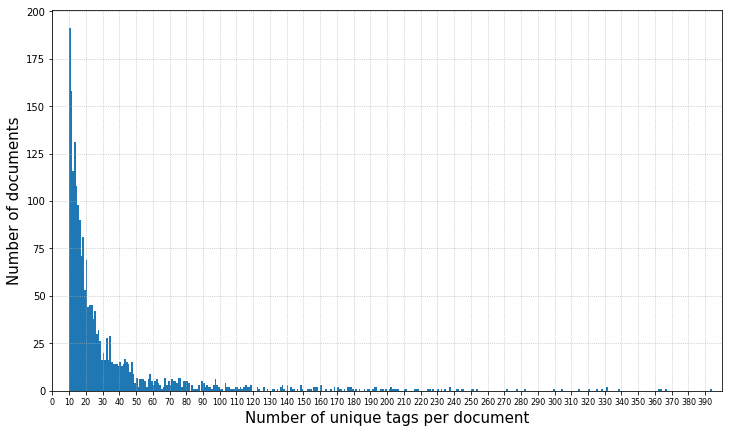
\includegraphics[width=\textwidth]{chapters/05_experiments/images/movielens_resources_per_tag.png}
    \caption{Distribution of the number of documents each tag was assigned to in the Movielens 20M + IMDB Synopses dataset (after pruning and preprocessing, not counting multiple assignments).}
    \label{fig:delicious_tag_doc_distr}
\end{figure}

\subsubsection{Construction and Preprocessing}

The first part of the dataset was obtained at https://grouplens.org/datasets/movielens/20m/. This download package includes a file with every tag assignment until October 17, 2016, for movies in the MovieLens website.

We preprocessed this dataset by normalizing all tags: lowercasing and removing special characters. In addition, we removed from the dataset all tags that occurred in less than 10 documents, following literature convention.

The download package includes a file that matches each MovieLens movie ID with the corresponding movie ID on the Internet Movie Database (IMDb) website \footnote{http://www.imdb.com/}. So, for each movie in the MovieLens dataset, its synopsis (when available) was manually scrapped from the IMDB website, using the \textit{Scrapy} \footnote{https://scrapy.org/} tool.

After crawling the website for the matching movie synopses, we saved the results and filtered out movies with non-english synopses.